\subsection{UC7 - Avvio del plug-in}
\begin{figure}[H]
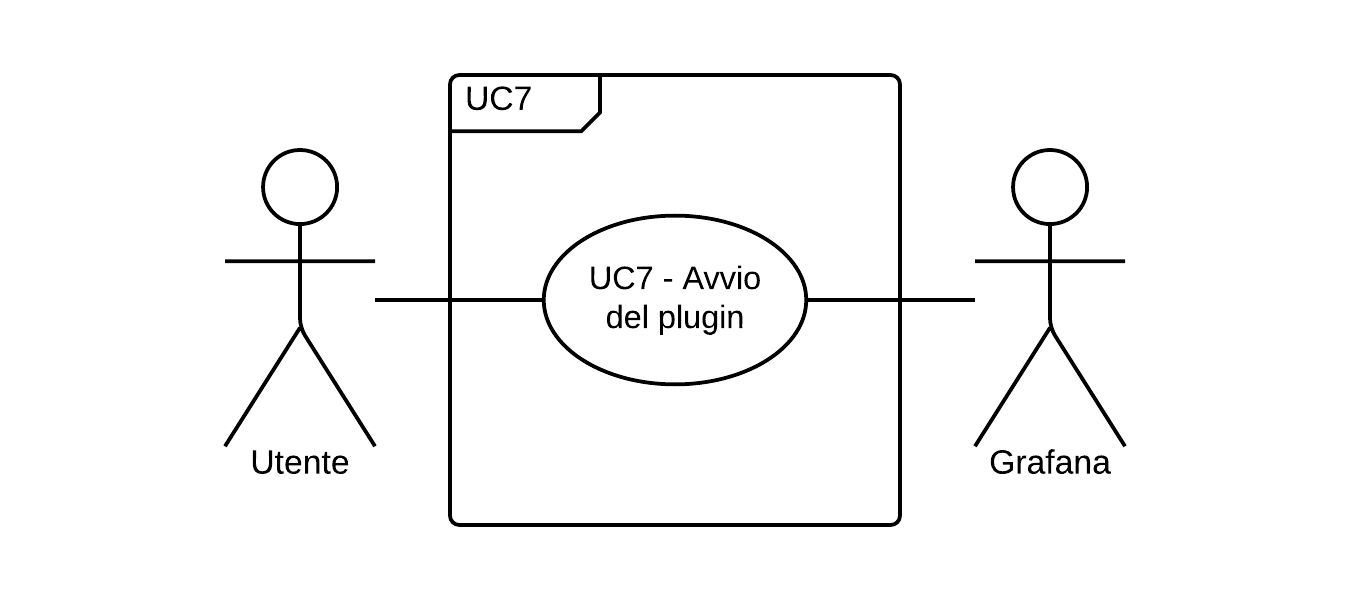
\includegraphics{img/UC7_-_Avvio_plugin.png}
\caption{Diagramma degli use case di UC7}
\end{figure}
\begin{itemize}
	\item \textbf{Codice identificativo}: UC7;
	\item \textbf{Titolo}: avvio del plug-in;
	\item \textbf{Attori primari}: utente;
	\item \textbf{Attori secondari}: Grafana\glo;
	\item \textbf{Descrizione}: l'utente esegue l'attività di avvio del plug-in che consiste nel suo collegamento ad una dashboard\glosp configurata;
	\item \textbf{Precondizioni}: l'utente è autenticato nel sistema software Grafana\glosp ed ha creato e configurato una dashboard\glosp per la visualizzazione del risultato;
	\item \textbf{Postcondizioni}: il plug-in è stato avviato correttamente;
	\item \textbf{Scenario principale}: l'utente accede alla dashboard\glosp e collega il plug-in. In questo modo esso viene avviato.
\end{itemize}
